\chapter{Control Design} \label{ch:control}
%ADD intro: in this section etc
Section \ref{sec:con.nlgc} introduces the concepts of Nonlinear Geometric Control, and the control design structure is discussed. 
The required control inputs are calculated by defining the tracking errors on nonlinear manifolds similar to the configuration spaces of the system dynamics.

%For the control of the different flight modes, the controllers are designed on the nonlinear geometric space, 
%being functions of the earlier described tracking errors. 
%Different flight modes are necessary to control the under-actuated system. 
A backstepping control approach is applied for the control of the load position tracking problem, allowing different controllers to operate in a cascaded structure. The controllers that are designed for each flight mode, are discussed in Section \ref{sec:con.track}. 

%ADD 
%deze references introduceren
%\cite{Bullo2005,Jurdjevic1997}

***************************************\\
%BART
bart: Descibe just as in chapter 2 what we are going to read in the next sections\\
nam: please check

***************************************\\

\section{Nonlinear Geometric Control}\label{sec:con.nlgc}
Many control systems are developed for the standard form of ordinary differential equations, namely $ \dot{x}=f(x,u) $, where the state and the control input are denoted by $ x $ and $ u $. It is assumed that the state and the control input lie in Euclidean spaces, and the system equations are defined in terms of smooth functions between Euclidean spaces. However, for many mechanical systems, the configuration space can only be expressed locally as a Euclidean space. In order to express the configuration space globally, a nonlinear space is required. A dynamical model on this nonlinear space is obtained in the previous chapter.

Geometric Control Theory is the study on how geometry of the state space influences controls problems. 
In control systems engineering, the underlying geometric features of a dynamic system are often not considered carefully. 
Differential geometric control techniques utilize these geometric properties for control system design and analysis.
The objective is to express both the system dynamics and control inputs on manifolds instead of local charts. 
In contrast to locally defined linear control, nonlinear geometric control can be defined almost globally, avoiding singularities that occur in the representation of large angles and complex maneuvering.

Global nonlinear dynamics of various classes of closed loop attitude control systems have been studied in recent years \cite{Chaturvedi2011a}.
In contrast to hybrid control systems \cite{Gillula2010}, complicated reachability set analysis is not required to guarantee safe switching between different flight modes, as the region of attraction for each flight mode covers the configuration space almost globally.


\paragraph{Backstepping Control}\label{sec:con.back}
A backstepping approach, or cascade control, is a Lyapunov based technique to design the control of nonlinear dynamical systems and ensures Lyapunov stability. 
This approach is commonly used for the control of \a{qr}s \cite{Mahony2012} and will also be used in this research for the control of the load trajectory tracking problem.\\
The basic principle is to create a cascaded structure by starting with a stable system as a base, then "stepping back" from this base to add a control loop around it that stabilizes the new system and enables the control of another state. 
This is repeated until the final external control is reached, see Figure \ref{fig:con.loop}.
The control law is designed by using states as virtual control signals. 
Each loop computes a virtual command signal for the adjacent inner loop. 
This backstepping approach determines how to stabilize the \a{qr} with the control inputs $ f $ and $ M $. 
The inner controller determines what the required control inputs are, driven by $ R_c $.  
The next controller calculates how to drive $ R_c $ based on $ q_c $, such that the \a{qr} is stabilized.
And the last controller determines which $ q_c $ is needed to follow the desired load position $ x_{L,d} $.

% CHECK nodig?
%\url{http://www.control.lth.se/media/Education/EngineeringProgram/FRTN05/2013/lec09_2013eight.pdf}
%We want to design a state feedback u=u(x) that stabilizes
%\begin{equation}\label{key}
%\begin{aligned}
%\dot{x}_1&=f(x_1)+g(x_1)x_2\\
%\dot{x}_2&=u
%\end{aligned}
%\end{equation}
%Idea is to see system as a cascade connection. Design controller first for inner loop, then for the outer.
%
%Back-Stepping Lemma
%\textbf{Lemma}: Let $ z=\begin{pmatrix}x_1,\cdots,x_{k-1}\end{pmatrix}^T$ and 
%\begin{equation}\label{key}
%\begin{aligned}
%\dot{z}&=f(z)+g(z)x_k\\
%\dot{x}_k&=u
%\end{aligned}
%\end{equation}
%Assume $ \phi(0)=0 $, $ f(0)=0 $,
%\begin{equation}\label{key}
%\dot{z}=f(z)+g(z)\phi(z)
%\end{equation}
%stable, and $ V(z) $ a Lyapunov function (with $ \dot{V}\leq-W $). Then, 
%\begin{equation}\label{key}
%u=\frac{d\phi}{dz}\begin{pmatrix}
%f(z)+g(z)x_k
%\end{pmatrix}-\frac{dV}{dz}g(z)-(x_k-\phi(z))
%\end{equation}
%stabilizes $ x=0 $ with $ V(z)+(x_k-\phi(z))^2/2 $ begin a Lyapunov function.
%
%The backstepping approach determines how to stabilize the {\displaystyle \mathbf {x} } \mathbf {x}  subsystem using {\displaystyle z_{1}} z_{1}, and then proceeds with determining how to make the next state {\displaystyle z_{2}} z_{2} drive {\displaystyle z_{1}} z_{1} to the control required to stabilize {\displaystyle \mathbf {x} } \mathbf {x} . Hence, the process "steps backward" from {\displaystyle \mathbf {x} } \mathbf {x}  out of the strict-feedback form system until the ultimate control {\displaystyle u} u is designed.
%***************************************\\

Because the \a{qr} has only four actuators, it is not possible to control all \a{DOF}s of the \a{qr}-Load system simultaneously. The backstepping approach allows control of different flight modes in which parts of the \a{DOF}s are controlled. The flight modes and their functions are defined in order, from the most inner loop to the most outer loop, as follows
\begin{outline}
\1 QR Attitude Controlled Mode 
\2 Track a desired QR attitude $ R_d(t) $ and a heading direction $ b_{1_d}(t) $
\2 Give a desired input $ M $ for system
\1 Load Attitude Controlled Mode 
\2 Track a desired load attitude command $ q_d(t) $
\2 Give a computed \a{qr} attitude $ R_c $ for the \a{qr} attitude controller (instead of $ R_d(t) $)
\1 Load Position Controlled Mode
\2 Track a desired load position $ x_{L,d}(t) $
\2 Give a computed load attitude $ q_c $ for the load attitude controller (instead of $q_d(t) $)
\end{outline}
where the subscript $d $ denotes a desired tracking reference, and the subscript $ c $ denotes a computed value that is calculated as a tracking reference. The difference in this notation is whether the signal is a predefined desired signal, or a signal computed by a controller.

%The controller that is used in this research is shown in Figure \ref{fig:con.loop}. The lowest levels have the highest bandwidth and are in control of the rotor rotational speeds $ \omega_i $, the total force $ f $ and moments $ M $. The next level controls the load attitude $ q $, and the top level controls the load position $ x_L $. 
\begin{figure}[h!]
	\centering
	\makebox[\textwidth][c]{\includegraphics[trim={0 0 0 9cm},clip,width=.95\textwidth]{./StyleStuff/backstepQR2.png}}
	\caption{Nonlinear Geometric Control Loop of the QR-Load system \cite{Sreenath2013c}\label{fig:con.loop}}
\end{figure}	

The design of the controllers for the \a{qr} attitude can be found in \cite{Lee2010}, and the controllers of load attitude- and position this can be found in \cite{Sreenath2013c}. Thorough stability analyses are presented in either references. For a deeper understanding of Lyapunov stability analysis in geometric control, the reader can refer to \cite{Bullo2005}.

\paragraph{Configuration Errors}\label{sec:con.errors}
The control system for a trajectory tracking problem requires state feedback and a measure of errors defined by a difference between the desired and current states.
The system dynamics evolve on nonlinear manifolds that describe the configuration spaces for the \a{qr} attitude $ \in SO(3) $ and the load attitude $ \in \mathbb{S}^2 $. 
Tracking errors functions are defined on these same manifolds, as shown in \cite{Bullo2005}, and form the basis of the controllers that must stabilize the \a{qr}-Load system.
%Likewise, the tracking errors $ \Psi_R:SO(3)\times SO(3)\rightarrow\mathbb{R} $ and $ \Psi_q:\mathbb{S}^2\times \mathbb{S}^2\rightarrow\mathbb{R} $ are expressed on these manifolds. 
%an for the purpose of control design. 
%The derivation of the error functions can be found in \cite{Bullo2005}.
 
%CHECK 
%\cite{Maithripala2006}

%CHECK
%Attitude control systems naturally evolve on nonlinear configuration spaces such as $ \mathbb{S}^2 $ and $ SO(3) $. 
%Attitude tracking control is developed on $ SO(3) $, therefore it avoids singularities of Euler-Angles.
Recall that $ R $ is the rotation matrix to describe the \a{qr} attitude, and $ R_d $ is the desired rotation matrix. To describe the relative rotation from the body frame to the desired frame, the attitude error is denoted as $ R^T_dR $. 
The \a{qr} attitude error function $ \Psi_R $ on $ SO(3) $ is chosen to be \cite{Lee2010c}
\begin{equation}\label{eq:psiR}
\Psi_R(R,R_d)=\frac{1}{2}tr\left[I-R_d^TR\right]
\end{equation}
such that $ \Psi_R $ is locally positive-definite about $ R^T_dR=I $ within the region where the rotation angle between $ R $ and $ R_d $ is less than $ 180^\circ $. 
It can be shown that this region where $ \Psi_R<2 $ almost covers $ SO(3) $.
%ADD explain
% instead of comparing all elements of rotation matrix. PsiR is a measure for the error
%ADD 
%(physical) Meaning of the error functions
Equation \ref{eq:mod.varRq} states that the variation of the rotation matrix is expressed as $ \delta R = R\hat{\eta} $ for $ \eta\in\mathbb{R}^3 $. Such that with Equation \ref{eq:mod.hatvee}, the derivative of Equation \ref{eq:psiR} is given by 
\begin{equation}\label{key}
\begin{aligned}
\mathbf{D}_R\Psi(R,R_d)\cdot R\hat{\eta}&=-\frac{1}{2}tr[R_d^TR\hat{\eta}]\\
&=\frac{1}{2}(R^T_dR-R^TR_d)^\vee\cdot\eta
\end{aligned}
\end{equation}
%By applying Equation \ref
%\texttt{\begin{equation}\label{key}
%\mathbf{D}_R\Psi(R,R_d)\cdot R\hat{\eta}=
%\end{equation}}
where the \textit{vee map} $ ^\vee:\mathfrak{so}(3)\rightarrow\mathbb{R}^3 $ is the inverse of the \textit{hat map} defined in Section \ref{sec:mod.geometric}. 
From this derivative, the attitude tracking error $ e_R $ is obtained 
\begin{equation}\label{eq:con.eR}
e_R=\frac{1}{2}(R_d^TR-R^TR_d)^\vee
\end{equation}
%The tracking error functions on $ TSO(3) $, the tangent space of $ SO(3) $, are defined as
%The attitude and angular velocity tracking error should be carefully chosen as they evolve on the tangent bundle of  $ SO(3) $. \cite{Lee2010c} 
It is important to note that the tangent vectors $ \dot{R} $ and $ \dot{R}_d $ cannot be compared directly, since they do not lie in the same space. $ \dot{R} $ and $ \dot{R}_d $ are expressed in their own tangent spaces, denoted by $ T_RSO(3)$ and $ T_{R_d}SO(3)$, respectively. For this reason, $ \dot{R}_d $ is transformed into a vector on $ T_RSO(3) $ to compare it with $ \dot{R} $. This is done by an mathematical object called a \textit{transport map}, which enables the comparison of velocities living in different spaces. See Figure \ref{fig:con.transport}, where two curves $ R(t), R_d(t)$ evolve on manifold $ SO(3) $, such that transport map $ \mathcal{T}(R,R_d):T_{R_d}SO(3)\mapsto T_RSO(3) $ allows comparison of $ \dot{R} $ and $ \dot{R}_d $.
\begin{figure}[h!]
	\centering
	\makebox[\textwidth][c]{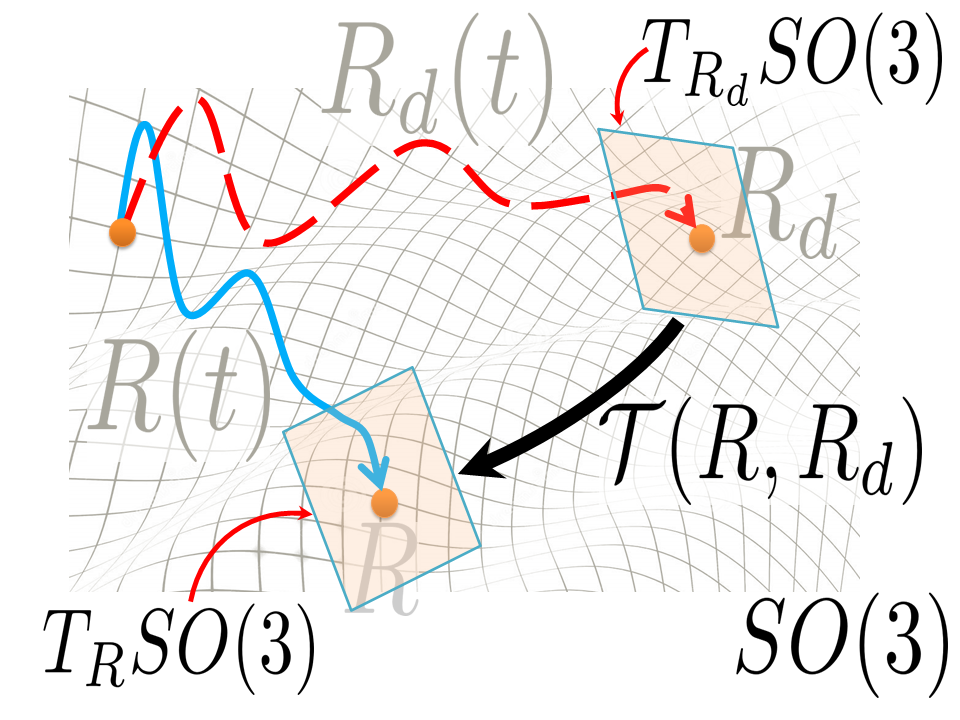
\includegraphics[width=.45\textwidth]{./StyleStuff/transport.png}}
	\caption{Transport map $ \mathcal{T}(R,R_d) $\label{fig:con.transport}}
\end{figure}		

%BUllo p536 transport maps
%BULLO Bullo p555 tracking error
%Substituting Equations \ref{eq:SO3} and \ref{eq:Rdot} into 
The comparison of the two tangent vectors is needed to calculate the error of body angular velocity $ \Omega $. This is derived from the velocity error that corresponds to the transport map $ \mathcal{T}(R,Rd)$, which is defined as
\begin{equation}\label{key}
\dot{e}=\dot{R}-\dot{R}_d(R_d^TR)
\end{equation}
This can be rewritten as follows
\begin{equation}\label{key}
\begin{aligned}
\dot{R}-\dot{R}_d(R_d^TR) &=R\hat{\Omega}-R_d\hat{\Omega}_d(R_d^TR) \\
&=R(\Omega)^\wedge-(RR^T)R_d\hat{\Omega}_dR_d^TR\\
&=R(\Omega)^\wedge-R(R^TR_d{\Omega}_d)^\wedge \\
&=R(\Omega-R^TR_d{\Omega}_d)^\wedge 
\end{aligned}
\end{equation}
From this follows the angular velocity tracking error $ e_{\Omega} $ in \BF, which  is defined as
\begin{align}\label{eq:con.eOmega}
e_\Omega&=\Omega- R^TR_d\Omega_d
\end{align}
Similar to the form of Equation \ref{eq:mod.R}, $ e_\Omega $ is the angular velocity vector of the relative rotation matrix $ R_d^TR $, represented in \BF. 
It can be shown that the following equation holds
\begin{equation}\label{key}
\frac{d}{dt}(R^T_dR)=(R_d^TR)\hat{e}_\Omega
\end{equation}

Next, the load attitude error function is expressed on $ \mathbb{S}^2 $ and represents the distance from the direction $ q $ to the desired direction $ q_d $. 
This is given by 
\begin{equation}\label{eq:psiq}
\Psi_q=1-q_d^Tq
\end{equation}

In the same fashion a \textit{transport map} is used for a comparison between the tangent vectors on tangent spaces $ T_q\mathbb{S}^2$ and $ T_{q_d}\mathbb{S}^2$. This results in the following error functions on $ T\mathbb{S}^2 $
\begin{align}
e_q&=\hat{q}^2q_d\label{eq:con.eq}\\
e_{\dot{q}}&=\dot{q}-(q_d\times\dot{q}_d)\times q\label{eq:con.edq}
\end{align}

The tracking errors for position and velocity are defined as
\begin{align}\label{key}
e_x&=x-x_d\\
e_v&=v-v_d
\end{align}
where $ v_d=\dot{x}_d $ and $ x_d(t) \in \mathbb{R}^3$ is a smooth desired load position.

\section{Tracking modes}\label{sec:con.track}
\subsection{Quadrotor Attitude Tracking}\label{sec:con.qratt}
The QR Attitude Controlled Mode is designed to control the \a{qr} attitude by tracking a smooth desired \a{qr} attitude command $ R_d(t) $.
This is done by controlling the earlier obtained error dynamics of $ e_R $ and $ e_\Omega $. The derivations of the equations in this section can be found in Section \ref{sec:app.error}.\\
From Equations \ref{eq:con.eR} and \ref{eq:con.eOmega}, the derivative of the attitude tracking error $ e_R $ can be written as
\begin{equation}\label{key}
\dot{e}_R=\frac{1}{2}(R_d^TR\hat{e}_\Omega+\hat{e}_\Omega R^TR_d)^\vee
\end{equation}

Similar to Equation \ref{eq:mod.R}, the kinematics equation for the desired attitude can be written as
\begin{equation}\label{eq:con.dotRd}
\dot{R}_d=R_d\hat{\Omega}_d \text{, and so } \hat{\Omega}_d=R_d^T\dot{R}_d
\end{equation}
The definition of the desired angular acceleration $ \dot{\Omega}_d $ can then be defined as follows
\begin{equation}\label{key}
\begin{aligned}
\dot{\hat{\Omega}}_d&=(\dot{R}_d^T\dot{R}_d)+(R_d^T\ddot{R}_d)\\
&=(R_d\hat{\Omega}_d)^T(R_d\hat{\Omega}_d)+(R_d^T\ddot{R}_d)\\
&=-\hat{\Omega}_d\hat{\Omega}_d+R_d^T\ddot{R}_d,\\
\dot{\Omega}_d&=(-\hat{\Omega}_d\hat{\Omega}_d+R_d^T\ddot{R}_d)^\vee
\end{aligned}
\end{equation}
From previous equations and Equations \ref{eq:mod.R}, \ref{eq:con.eOmega} and the fact that $ \hat{\Omega}_d\Omega_d =0$, follows that the derivative of the angular velocity tracking error $ e_\Omega $ can be written as 
\begin{equation}\label{eq:con.deOmega}
\dot{e}_\Omega=\dot{\Omega}+\hat{\Omega}R^TR_d\Omega_d-R^TR_d\dot{\Omega}_d
%\dot{e}_\Omega=J^{-1}(-\Omega\times J\Omega + M)+\hat{\Omega}R^TR_d\Omega_d-R^TR_d\dot{\Omega}_d
\end{equation}
By substituting Equation \ref{eq:mod.qratt} follows
\begin{equation}\label{eq:con.dOmega}
\dot{e}_\Omega=J^{-1}(-\Omega\times J\Omega + M)+\hat{\Omega}R^TR_d\Omega_d-R^TR_d\dot{\Omega}_d
\end{equation}

Now the control input $ M $ can be defined as a proportional term, a derivative term and a canceling term, as follows \cite{Sreenath2013c}
\begin{equation}\label{eq:con.M}
M = -k_Re_R-k_\Omega e_\Omega+\Omega\times J\Omega-J(\hat{\Omega}R^TR_d\Omega_d-R^TR_d\dot{\Omega}_d)
\end{equation}
such that Equation \ref{eq:con.deOmega} is reduced to
\begin{equation}\label{eq:con.JdeOmega}
J\dot{e}_\Omega=-k_Re_R-k_\Omega e_\Omega
\end{equation}
for any positive constants $ k_R, k_\Omega $.
In \cite{Sreenath2013b}, Equation \ref{eq:con.M} is defined as
\begin{equation}\label{eq:con.Meps}
M = -\frac{1}{\epsilon^2}k_Re_R-\frac{1}{\epsilon}k_\Omega e_\Omega+\Omega\times J\Omega-J(\hat{\Omega}R^TR_d\Omega_d-R^TR_d\dot{\Omega}_d)
\end{equation}
where \lsymb{$ \epsilon $}{Tuning parameter to enable rapid exponential convergence of $ e_R, e_\Omega $} is a parameter to enable rapid exponential convergence of the attitude- and angular velocity error functions, such that $ 0<\epsilon<1 $.\\
%%ADD waarom?
%%CHECK waar moet dit
%It can be shown that $ \parallel\dot{e}_R\parallel\leq\parallel e_\Omega \parallel  $ for all $ R^T_dR\in SO(3) $.
 
A stability analysis of the controller is presented in \cite{Lee2010} and it is proven that the zero equilibrium of the closed loop tracking error $ (e_R,e_\Omega)=(0,0) $ is exponentially stable, if the initial conditions satisfy
\begin{equation}\label{eq:dom1}
\Psi_R(R(0),R_d(0))<2
\end{equation}
\begin{equation}\label{eq:dom2}
\parallel e_\Omega(0)\parallel^2<\frac{2}{\lambda_M(J)}\frac{k_R}{\epsilon^2}(2-\Psi_R(R(0),R_d(0)))
\end{equation}
where \lsymb{$ \lambda_M(\cdot) $}{Maximum eigenvalue} denotes the maximum eigenvalue. The domain of attraction is defined by Equations \ref{eq:dom1} and \ref{eq:dom2}. \\
Furthermore, there exist constants $ \alpha_R,\beta_R>0 $ such that
\begin{equation}\label{eq:con.PsiRconv}
\Psi_R(R(t),R_d(t)) \leq min\left\lbrace 2,\alpha_Re^{-\beta_Rt}\right\rbrace 
\end{equation}
%ADD explain that error function will be asymptoticallly stable for right parameters. larger region of attraction

%CHECK what this is about
%Asymptotic tracking of the quadrotor attitude does not require specification of the thrust magnitude. As an auxiliary problem, the thrust magnitude can be chosen in many different ways to achieve an additional translational motion objective. For example, it can be used to asymptotically track a quadrotor altitude command [28]. Since the translational motion of the quadrotor UAV can only be partially controlled; this flight mode is most suitable for short time periods where an attitude maneuver is to be completed. \cite{Goodarzi2015b}

%CHECK waar moet dit?
\begin{equation}\label{key}
J\dot{e}_\Omega=-\frac{1}{\epsilon^2}k_Re_R-\frac{1}{\epsilon}k_\Omega e_\Omega
\end{equation} 

\subsection{Load Attitude Tracking}\label{sec:con.loadatt}

%ADD How is the controller built.
%CHECK nodig? Net als bij M, hoe komen ze hier op?
%A control input is composed of a proportional term along the gradient of $ \Psi_q $, a derivative term and a cancellation term.
%\begin{equation}\label{key}
%u=mL^2(-k_qq_d\times q-k_{\omega}\omega-\frac{g}{L}q\times e_3)
%\end{equation}


%ADD Dependent of what values? 	How to choose parameters.

%\begin{figure}[h!]
%	\centering
%	\makebox[\textwidth][c]{\includegraphics[width=.45\textwidth]{./StyleStuff/dcsc.png}}
%	\caption{\label{fig:con.loadattloop}}
%\end{figure}		

The Load Attitude Controlled Mode tracks a desired load attitude $ q_d $ by calculating a command signal for the \a{qr} attitude, defined as
\begin{equation}\label{eq:con.R}
R_c = \begin{bmatrix}
b_{1c}; b_{3c}\times b_{1c};b_{3c}
\end{bmatrix}
\end{equation}
where $ b_{3c} \in \mathbb{S}^2 $ is defined by 
\begin{equation}\label{eq:con.b3c}
b_{3c}=\frac{F}{||F||}
\end{equation}
Such that $ F $ in Equation \ref{eq:con.b3c} is defined by a normal component $ F_n $, $ F_{pd} $ and $ F_{ff}$
\begin{equation}\label{key}
F=F_n-F_{pd}-F_{ff}
\end{equation}
 Control forces for a system evolving on $ \mathbb{S}^2 $, are derived in \cite{Bullo2005}. 
 This results in a proportional-derivative force $ F_{pd} $ and a feed forward force $ F_{ff} $, that are functions of Equations \ref{eq:con.eq} and \ref{eq:con.edq}. The following terms are obtained
\begin{equation}\label{key}
\begin{aligned}
F_{pd}&=-k_P\hat{q}^2q_d-k_D(\dot{q}-(q_d\times\dot{q}_d\times q)\\
&=-k_qe_q-k_\omega e_{\dot{q}}
\end{aligned}
\end{equation}
\begin{equation}\label{key}
F_{ff}=m_QL\langle\langle q,q_d\times\dot{q}_d\rangle\rangle_{\mathbb{R}^3}(q\times \dot{q})+m_QL(q_d\times \ddot{q}_d)\times q
\end{equation}
The unit vector $ b_{1c} $ is defined as \cite{Lee2010d}
\begin{equation}\label{key}
b_{1c}=-\frac{1}{||b_{3c}\times b_{1d}||}(b_{3c}\times(b_{3c}\times b_{1d}))
\end{equation}
where $ b_{1d}\in \mathbb{S}^2 $ is chosen, not parallel to $ b_{3c} $.
The total upward thrust is defined as
\begin{equation}\label{key}
f=F\cdot Re_3
\end{equation}

%ADD explain that error function will be asymptoticallly stable for right parameters. larger region of attraction
It is proven in \cite{Sreenath2013c} that the zero equilibrium of the closed loop tracking error $ (e_q,e_{\dot{q}},e_R,e_\Omega)=(0,0,0,0) $ is exponentially stable, if the initial conditions satisfy
\begin{equation}\label{eq:dom3}
\Psi_q(q(0),q_d(0))<2
\end{equation}
\begin{equation}\label{eq:dom4}
\parallel e_{\dot{q}}(0)\parallel^2<\frac{2}{m_QL}{k_R}(2-\Psi_q(q(0),q_d(0)))
\end{equation}

The domain of attraction is defined by Equations \ref{eq:dom1}, \ref{eq:dom2}, \ref{eq:dom3} and \ref{eq:dom4}.
Furthermore, there exist constants $ \alpha_q,\beta_q>0 $ such that
\begin{equation}\label{eq:con.Psiqconv}
\Psi_q(q(t),q_d(t)) \leq min\left\lbrace 2,\alpha_qe^{-\beta_qt}\right\rbrace 
\end{equation}

\subsection{Load Position Tracking}\label{sec:con.loadpos}

%CHECK nodig?
%Explain how $ f $ and $ \vec{b_{1_d}} $ is obtained from $ x_d(t) $?\\

Tracks load position reference. Outputs load attitude reference.

\begin{equation}\label{eq:con.q}
q_c = - \frac{A}{||A||}
\end{equation}
where
\begin{equation}\label{key}
A = -k_xe_x-k_ve_v+(m_Q+m_L)(\ddot{x}_{L,d}+ge_3)+m_QL(\dot{q}\cdot\dot{q})q
\end{equation}
with $ e_x=x_L-x_{L,d} $ and $ e_v=\dot{x}_L-\dot{x}_{L,d} $.
Furthermore, $ F_n $ is redefined as
\begin{equation}\label{key}
F_n=(A\cdot q)q
\end{equation}
%\begin{figure}[h!]
%	\centering
%	\makebox[\textwidth][c]{\includegraphics[width=.45\textwidth]{./StyleStuff/dcsc.png}}
%	\caption{\label{fig:con.loadposloop}}
%\end{figure}		

%CHECK error function will be asymptoticallly stable for right parameters? 
It is proven in \cite{Sreenath2013c} that the zero equilibrium of the closed loop tracking error $ (e_x,e_v,e_q,e_{\dot{q}},e_R,e_\Omega)=(0,0,0,0,0,0) $ is exponentially stable, if the initial conditions satisfy
\begin{equation}\label{eq:dom5}
\Psi_q(q(0),q_c(0))<\psi_1<1
\end{equation}
\begin{equation}
\parallel e_{x}(0)\parallel^2<e_{x_{max}}
\end{equation}
where $ e_{x_{max}} $ and $ \psi_1 $ are fixed design depended constants. 

The domain of attraction is defined by Equations \ref{eq:dom1}, \ref{eq:dom2}, \ref{eq:dom5} and the following equation
\begin{equation}
\parallel e_{\dot{q}}(0)\parallel^2<\frac{2}{m_QL}{k_q}(\psi_1-\Psi_q(q(0),q_d(0)))
\end{equation}


Furthermore, there exist constants $ \alpha_q,\beta_q>0 $ such that
\begin{equation}\label{key}
\Psi_q(q(t),q_d(t)) \leq min\left\lbrace 2,\alpha_qe^{-\beta_qt}\right\rbrace 
\end{equation}

\section{Stability Analysis}\label{sec:con.sta}

Normally Lyapunov Analysis is 


Lyapunov Analysis on SO3 x R3 and S2 x R3

Closed-loop full-attitude dynamics evolve on the non-Euclidean manifold $ SO(3) \times \mathbb{R}^3 $. 
Since these manifolds are locally Euclidean, local stability properties of a closed-loop equilibrium solution can be assessed using standard Lyapunov methods. In addition, the LaSalle invariance result and related Lyapunov results apply to closed-loop vector fields defined on these manifolds. 

However, since the manifolds $ SO(3) $ and $ \mathbb{S}^2 $ are compact, the radial unboundedness assumption cannot be satisfied; consequently, global asymptotic stability cannot follow from a Lyapunov analysis on Euclidean spaces [40], and therefore must be analyzed in alternative ways [19]–[23].\cite[p.43]{Chaturvedi2011}

[40]:
[19]:
[20]:
[21]:
[22]:
[23]:


\cite{Chaturvedi2011} summarizes global results on attitude control and stabilization for a rigid body using continuous time- invariant feedback. The analysis uses methods of geometric mechanics based on the geometry of the special orthogonal group $ SO(3) $ and the two-sphere $ \mathbb{S}^2 $.

%ADD 
%Justify choice of parameters. Up to what level can we push the system? Where can we find more info about domain of attractions.
%How to choose parameters and how to select gains for errors

***************************************\\
%BART 
Bart: Ok, but what are you doing with this? Does this relate to backstepping?\\
Nam: Dit gaat over analyse die je normaal doet mbv Lyapunov om de stabiliteit aan te tonen. 

***************************************\\


***************************************\\
%BART
Bart: Does this include a part about tuning of the controller?\\
Nam: De stabiliteit hangt wel samen met de control parameters. De keuze hiervan is op dit moment arbitrair. De 'juiste' gains kiezen is wellicht zoals eerder besproken overbodig 

***************************************\\

%HOeft waarschijnlijk niet eens een section te zijn, kan kort en bondig
\section*{Summary}

%ADD What is Geometric Control? Differences between other control
In this chapter the control design based on Nonlinear Geometric Control was discussed.

The main difference with other control techniques is that the tracking errors are also defined on manifolds, which allows the design of almost global defined controllers.

Stability analysis is different from a Lyapunov analysis on Euclidean spaces.
%This fact is 

%ADD Why Geometric Control? Why is useful
%PRO
%The proposed control system is robust to switching conditions since each flight mode has almost global stability properties, and it is straightforward to design a complex maneuver of a QR. \cite{Lee2010c}

In order to test the control performance of a load position tracking objective, experiments are defined in the next chapter. 




